\section{\textit{Graphical Analysis}}
        
    \subsection{\textit{Graphs of Magnetic field versus Current in relation to the value of the permeability of free space}}
    
        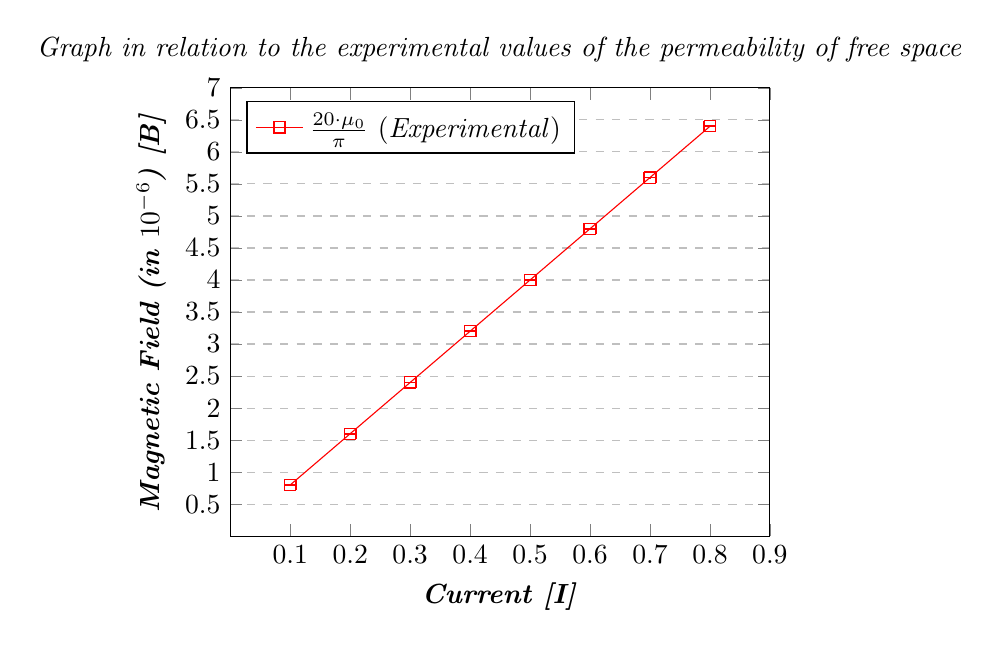
\begin{tikzpicture}
            \begin{axis}[
                title={\textit{Graph in relation to the experimental values of the permeability of free space}},
                xlabel={\textbf{\textit{Current [I]}}},
                ylabel={\textbf{\textit{Magnetic Field (in \bm{$10^{-6}$}) [B]}}},
                xmin=0, xmax=0.9,
                ymin=0, ymax=7,
                xtick={0.1,0.2,0.3,0.4,0.5,0.6,0.7,0.8,0.9},
                ytick={0.5,1,1.5,2,2.5,3,3.5,4,4.5,5,5.5,6,6.5,7,7.5,8},
                legend pos=north west,
                ymajorgrids=true,
                grid style=dashed,
                legend entries={$\frac{20\cdot\mu_0}{\pi}$ (\textit{Experimental})}
            ]
            
            \addplot+[
                color=red,
                mark=square,
                ] plot[error bars/.cd, y dir=both, y explicit, x dir=both, x explicit]
                coordinates {
                (0.1,0.8) +- (0.01,0.005)
                (0.2,1.6) +- (0.01,0.005)
                (0.3,2.4) +- (0.01,0.005)
                (0.4,3.2) +- (0.01,0.005)
                (0.5,4.0) +- (0.01,0.005)
                (0.6,4.8) +- (0.01,0.005)
                (0.7,5.6) +- (0.01,0.005)
                (0.8,6.4) +- (0.01,0.005)
                };
                
            \end{axis}
        \end{tikzpicture}
        
        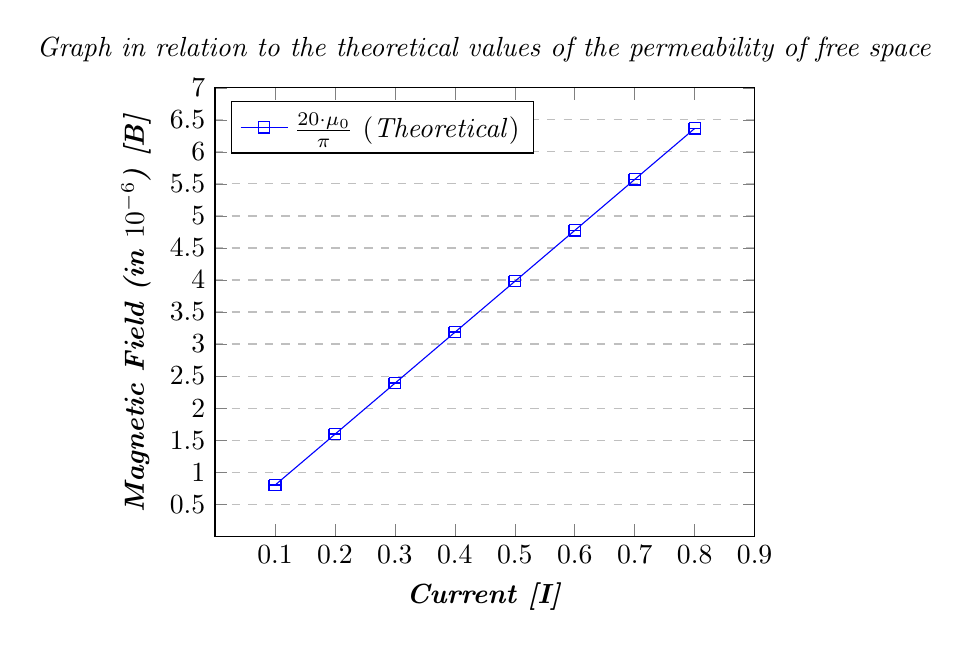
\begin{tikzpicture}
            \begin{axis}[
                title={\textit{Graph in relation to the theoretical values of the permeability of free space}},
                xlabel={\textbf{\textit{Current [I]}}},
                ylabel={\textbf{\textit{Magnetic Field (in \bm{$10^{-6}$}) [B]}}},
                xmin=0, xmax=0.9,
                ymin=0, ymax=7,
                xtick={0.1,0.2,0.3,0.4,0.5,0.6,0.7,0.8,0.9},
                ytick={0.5,1,1.5,2,2.5,3,3.5,4,4.5,5,5.5,6,6.5,7,7.5,8},
                legend pos=north west,
                ymajorgrids=true,
                grid style=dashed,
                legend entries={$\frac{20\cdot\mu_0}{\pi}$ (\textit{Theoretical})}
            ]
            
            \addplot+[
                color=blue,
                mark=square,
                ] plot[error bars/.cd, y dir=both, y explicit, x dir=both, x explicit]
                coordinates {
                (0.1,0.796) +- (0.01,0.005)
                (0.2,1.591) +- (0.01,0.005)
                (0.3,2.387) +- (0.01,0.005)
                (0.4,3.183) +- (0.01,0.005)
                (0.5,3.978) +- (0.01,0.005)
                (0.6,4.774) +- (0.01,0.005)
                (0.7,5.570) +- (0.01,0.005)
                (0.8,6.366) +- (0.01,0.005)
                };
                
            \end{axis}
        \end{tikzpicture}
        
        \textit{Upon close visual observation, we see that the difference in the plotted values of that of the theoretical and experimental values of the permeability of free space from the B-I graph are very minute to the extent that it would be right to say and consider that the experimental values are both accurate and precise in relation to that of the literature or theoretical values of the permeability of free space.}
        
    \subsection{\textit{Graphs of Magnetic field versus Current in relation to the value of the permittivity of free space}}
    
        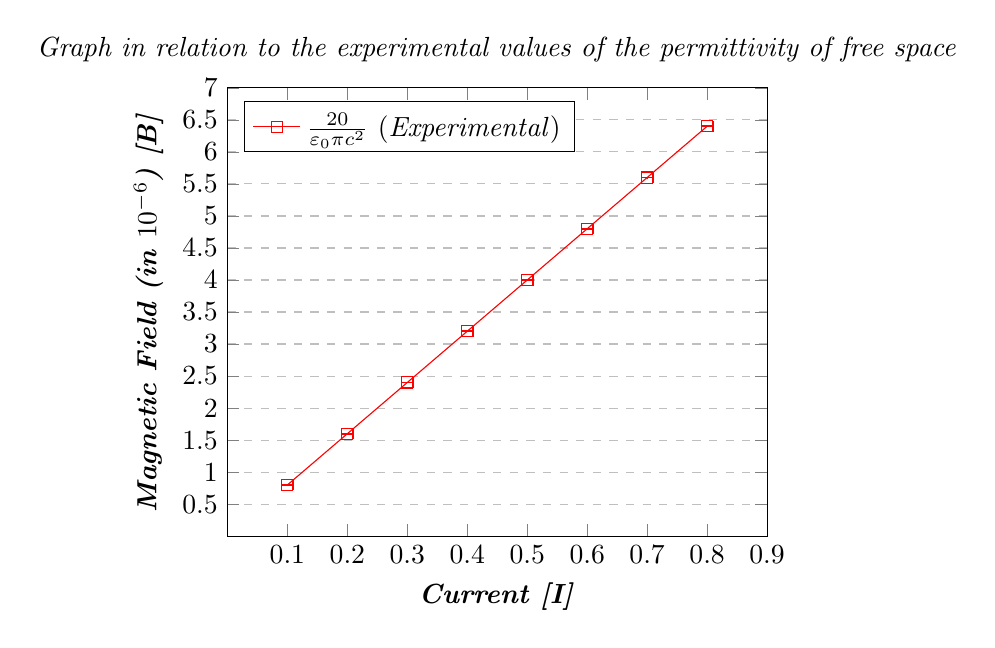
\begin{tikzpicture}
            \begin{axis}[
                title={\textit{Graph in relation to the experimental values of the permittivity of free space}},
                xlabel={\textbf{\textit{Current [I]}}},
                ylabel={\textbf{\textit{Magnetic Field (in \bm{$10^{-6}$}) [B]}}},
                xmin=0, xmax=0.9,
                ymin=0, ymax=7,
                xtick={0.1,0.2,0.3,0.4,0.5,0.6,0.7,0.8,0.9},
                ytick={0.5,1,1.5,2,2.5,3,3.5,4,4.5,5,5.5,6,6.5,7,7.5,8},
                legend pos=north west,
                ymajorgrids=true,
                grid style=dashed,
                legend entries={$\frac{20}{\varepsilon_0\pi c^2}$ (\textit{Experimental})}
            ]
            
            \addplot+[
                color=red,
                mark=square,
                ] plot[error bars/.cd, y dir=both, y explicit, x dir=both, x explicit]
                coordinates {
                (0.1,0.8) +- (0.01,0.005)
                (0.2,1.6) +- (0.01,0.005)
                (0.3,2.4) +- (0.01,0.005)
                (0.4,3.2) +- (0.01,0.005)
                (0.5,4.0) +- (0.01,0.005)
                (0.6,4.8) +- (0.01,0.005)
                (0.7,5.6) +- (0.01,0.005)
                (0.8,6.4) +- (0.01,0.005)
                };
                
            \end{axis}
        \end{tikzpicture}
        
        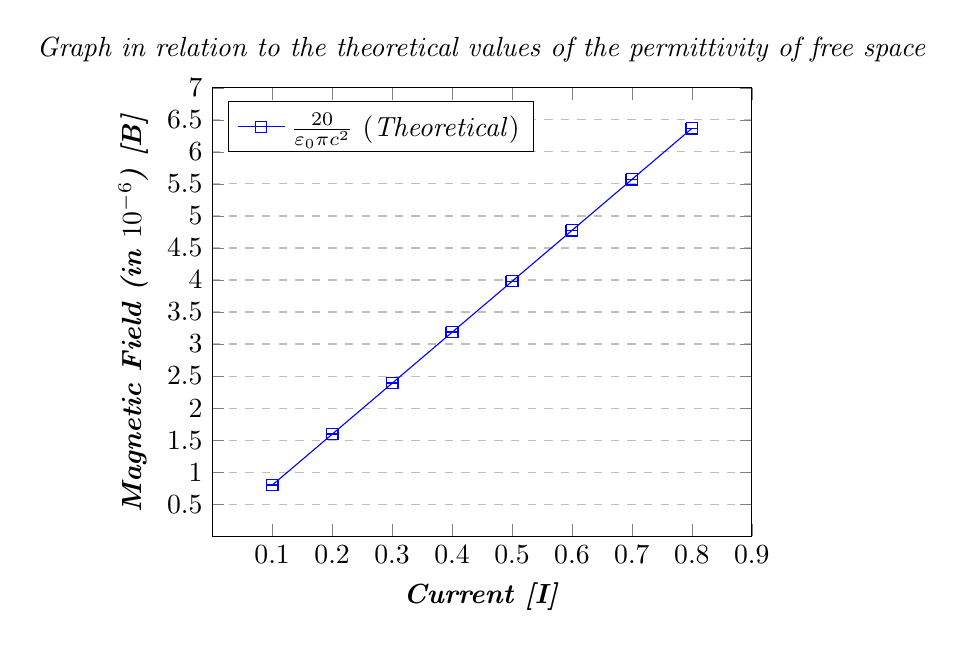
\begin{tikzpicture}
            \begin{axis}[
                title={\textit{Graph in relation to the theoretical values of the permittivity of free space}},
                xlabel={\textbf{\textit{Current [I]}}},
                ylabel={\textbf{\textit{Magnetic Field (in \bm{$10^{-6}$}) [B]}}},
                xmin=0, xmax=0.9,
                ymin=0, ymax=7,
                xtick={0.1,0.2,0.3,0.4,0.5,0.6,0.7,0.8,0.9},
                ytick={0.5,1,1.5,2,2.5,3,3.5,4,4.5,5,5.5,6,6.5,7,7.5,8},
                legend pos=north west,
                ymajorgrids=true,
                grid style=dashed,
                legend entries={$\frac{20}{\varepsilon_0\pi c^2}$ (\textit{Theoretical})}
            ]
            
            \addplot+[
                color=blue,
                mark=square,
                ] plot[error bars/.cd, y dir=both, y explicit, x dir=both, x explicit]
                coordinates {
                (0.1,0.796) +- (0.01,0.005)
                (0.2,1.591) +- (0.01,0.005)
                (0.3,2.387) +- (0.01,0.005)
                (0.4,3.183) +- (0.01,0.005)
                (0.5,3.978) +- (0.01,0.005)
                (0.6,4.774) +- (0.01,0.005)
                (0.7,5.570) +- (0.01,0.005)
                (0.8,6.366) +- (0.01,0.005)
                };
                
            \end{axis}
        \end{tikzpicture}
        
        \textit{Upon close visual observation, we see that the difference in the plotted values of that of the theoretical and experimental values of the permittivity of free space from the B-I graph are very minute to the extent that it would be right to say and consider that the experimental values are both accurate and precise in relation to that of the literature or theoretical values of the permittivity of free space.}

